\documentclass{article}
\newtheorem{thm}{Theorem}
\setlength{\oddsidemargin}{0.25in}
\setlength{\textwidth}{6in}
\setlength{\topmargin}{-0.25in}
\setlength{\headheight}{0.3in}
\setlength{\headsep}{0.2in}
\setlength{\textheight}{9in}
\setlength{\footskip}{0.1in}
\usepackage{multirow}
\usepackage{fullpage}
\usepackage{graphicx}
\usepackage{amsthm}
\usepackage{amssymb}
\usepackage{url}
\usepackage{amsfonts}
\usepackage{algpseudocode}
\usepackage{mathtools}
\begin{document}\title{Homework 2\\ Computer Science \\ Fall 2016\\ B565}         % Enter your title between curly braces
\author{Professor Dalkilic}        % Enter your name between curly braces
\date{\today}          % Enter your date or \today between curly braces
\maketitle
\makeatother     % `@' is restored as a "non-letter" character
\pagestyle{plain}
\section*{Directions}
Please follow the syllabus guidelines in turning in your homework.  I will provide the \LaTeX{} of this document too.  You may use it or create one of your own.  This homework should be started quickly.   Sometimes there are natural questions arising from code.  Within a week, AIs can contact students to examine code; students must meet within three days.  The session will last no longer than 5 minutes.  If the code does not work, the grade for the program may be reduced.  Lastly, source code cannot be modified post due date.

\section*{$k$-means Algorithm in Theory}
This part of the problem asks you to reflect on $k$-means and work through its theoretical elements.  I have written algorithm below.   Answer the subsequent questions.

{\small
\begin{center}
\begin{algorithmic}[1]\label{kmeans}
\State{\bf ALGORITHM} \texttt{k-means}
\State {\bf INPUT} (\textsf{data} $\Delta$, distance $d:\Delta^2\rightarrow \mathbb{R}_{\geq 0}$, \textsf{centoid number} $k$, \textsf{threshold} $\tau$)
\State {\bf OUTPUT} (\textsf{Set of centoids} $\{c_1, c_2, \ldots, c_k\}$)
\State
\State \texttt{***} $Dom(\Delta)$ denotes domain of data.
\State
\State \texttt{***} Assume centroid is structure $c = (v \in DOM(\Delta), B\subseteq \Delta)$
\State  \texttt{***} $c.v$ is the centroid value and $c.B$ is the set of nearest points.
\State \texttt{***}  $c^{i}$ means centroid at $i^{th}$ iteration. 
\State
\State $i = 0$
\State \texttt{***} Initialize Centroids
\For{$j = 1,k$}
\State $c_j^i.v \gets  random(Dom(\Delta))$
\State $c_j^i.B \gets \emptyset$
\EndFor
\State
\Repeat
\State $i \gets i + 1$
\State \texttt{***} Assign data point to {\it nearest} centroid
\For {$\delta \in \Delta$}
\State $c_j^i.B \gets c.B \cup \{\delta\}$, where $\min_{c_j^i}\{d(\delta, c_j^i.v)\}$
\EndFor
\For {$j = 1, k$}
\State \texttt{***} Get size of centroid
\State $n \gets |c_j^i.B|$
\State \texttt{***} Update centroid with average 
\State $c_j^i.v \gets (1/n)\sum_{\delta \in c_j^i.B} \delta$
\State \texttt{***} Remove data from centroid
\State $c_j^i.B \gets \emptyset$
\EndFor
\State \texttt{***} Calculate scalar product (abuse notation and structure slightly)
\State \texttt{***} See notes
\Until{$((1/k)\sum_{j=1}^k~|| c^{i-1}_j-c^{i}_j||) < \tau$}
\State {\bf return} ($\{c_1^i, c_2^i, \ldots, c_k^i\}$) 
\end{algorithmic}
\end{center}}
\subsection*{$k$-means on a tiny data set.}
Here are the inputs:
\begin{eqnarray}
\Delta &=& \{  (2, 5),  (1,5) , (22, 55), (42, 12), (15,16)\}\\
d((x_1, y_1) ,(x_2, y_2)) &=& [(x_1-x_2)^2 + (y_1 - y_2)^2)]^{1/2}\\
k &=&2\\
\tau &=& 10
\end{eqnarray}

Observe that $Dom(\Delta) = \mathbb{R}^2$.  We now work through $k$-means. We ignore the uninformative assignments.  We remind the reader that $\mathsf{T}$ means transpose.

\begin{center}
\begin{algorithmic}[1]
\State $i \gets 0$
\State \texttt{***} Randomly assign value to first centroid.
\State $c^0_1.v \gets random(Dom(\Delta)) = (16,19)$
\State \texttt{***} Randomly assign value to second centroid.
\State $c^0_2.v \gets random(Dom(\Delta)) = (2,5)$
\State $i \gets i + 1$
\State \texttt{***} Associate each datum with nearest centroid
\State $c^1_1.B = \{(22, 55), (42, 12), (15,16)\}$
\State $c^1_2.B = \{(2,5), (1,5)\}$
\State \texttt{***} Update centroids
\State $c^1_1.v \gets (26.3, 27.7) = (1/3)((22,55) + (42,12) + (15,16))$
\State $c^1_2.v \gets (1.5, 5) = (1/2)((2,5) + (1,5))$
\State \texttt{***} The convergence condition is split over the next few lines to explicitly show the calculations
\State $(1/k)\sum_{j=1}^k~|| c^{i-1}_j-c^{i}_j|| = (1/2)(||c^0_1 - c^1_1||+ ||c^0_2 - c^1_2||) = (1/2) (||{2 \choose 5} - {1.5 \choose 5}|| + ||{16 \choose 19} - {26.3 \choose 27.7}||)$
\State $ = (1/2)[({.5 \choose 0}^{\mathsf{T}}{.5 \choose 0})^{(1/2)} + ({-9.7 \choose  -8.7}^{\mathsf{T}}{-9.7 \choose  -8.7})^{(1/2)})] = (1/2)(\sqrt{.5} + \sqrt{169.7}) \sim (1/2)(13.7) = 6.9$
\State Since the threshold is met $(6.9 < 10)$, $k$-means stops, returning $\{(26.3, 27.7), (1.5,5)\}$
\end{algorithmic}
\end{center}



\subsection*{Questions}

\begin{enumerate}
\item Does $k$-means always converge? Given your answer, a bound on the iterate must be included.  How is its value determined? \\
Ans) No, there are scenarios where K-means may not converge properly. Convergence of k-means mostly depends on choosing the right centroids for given data. WE can take a bound of the number of times above algorithm can run and print the convergence obtained by running our code and check if its decreasing for each iteration. Based on this we can make sure convergence of k-means occurs.
\item \textsc{Lines} 12-16 of the $k$-means algorithm describe initialization of the centroids.  Why is this code problematic?  What are some implications of using $k$-means?    \\ 
Ans) Based on the way we are choosing the centroids there can be a centroid collision(two or mode centroids are same) or centroid ties may occur.. This might lead to undesirable results.
\item What is the run-time of this algorithm (include your new parameter from Question 1). \\
  \textbf{ Write an answer for this one.} 
  
\item We describe two problems that arise when using $k$-means in practice.  Assume the datum is $\delta\in\Delta$, the centroids are $c_i, c_j$ for $i\neq j$ and distance $d$.  
\begin{itemize}
\item {\it Ties} occur when $d(c_i, \delta) = d(c_j, \delta)$.  Of course, there can be threeway, fourway, $\ldots$, $k$-way ties.  One solution is to randomly assign the datum to one of the two centroids.   What are two other solutions to this problem? \\
Ans) 2nd solution is to add the datum to all the centroid having ties for this iteration. \\
3rd solution is to ignore the datum completly in this iteration and consider it normally from next partition.
\item {\it Centroid collapse} occurs when $d(c_i, c_j) \sim 0$. Like ties, this can include more than two.  One is to find the median $m$ of the union of the two centroids and then assign values less than the median to one and values greater than the median to the other, taking into account an odd number will be the problem above.  What are two other solutions?  Observe that an additional threshold on centroids, $\tau_c > 0$, is needed, to determine whether $d(c_i, c_j) \leq \tau_c$ is true.  First, how would $\tau_c$ be determined?  Second, where in the algorithm should this be checked? \\
Ans) second solution is to find the mean $m$ of the union of the two centroids and then assign values less than the mean to one and values greater than the mean to the other \\
third solution is to find the mode $m$ of the union of the two centroids and then assign values less than the mode to one and values greater than the mode to the other. We can also randomly choose a new point to one of the centroid and recheck if all the centroids untill we dont have any centroid collisions.\\

\item Modify the $k$-means algorithm to address ties and collapsing centroids.  Explicitly add pseudo-code to the algorithm and call this $k$-meansr. 
 	\\
\end{itemize}
\end{enumerate}

\subsection*{Integration}
We will look at the problem of integrating two pieces of data through a metric.  The data are described by $([X:t], d_x), ([Y:u], d_u)$ where $X:t$ means it is type $t$,  $Y:u$ is type $u$, and $d_x,d_y$ distance metrics.  We integrate the data and now need a metric $([X:t]\times [Y:u], d)$.  Is this possible?  We need to prove  that $d$ is a metric.  To make notation easier, assume $Z = [X:t]\times [Y:u]$.  For $(a,b) \in Z^2$, we write $a_0$ to mean the $t$ type leftside of the product and $b_0$ for the $t$ type rightside.  For example, $Z = [N : \textsf{int}] \times [S : \textsf{string}]$.  $(a,b) = ((34, \texttt{two}), (100, \texttt{three}))$, then $a_0 = 34, b_0 = 100$ and $a_1 = \texttt{two}, b_1 = \texttt{three}$.

Let's define one of the simplest metrics.
$d:Z^2 \rightarrow \mathbb{R}_{\geq 0}$ where:
\begin{eqnarray*}
d(a,b) &=& d_x(a_0,b_0) + d_y(a_1,b_1)
\end{eqnarray*}
Now we show reflexivity, symmetry, and transitivity.  
\begin{itemize}
\item $(\forall, a \in Z)\ d(a,a) = 0$.  Then $d(a,a) = d_x(a_0,a_0) + d_y(a_1,a_1) = 0$  
\item $(\forall\, a, b)\ d(a,b) \rightarrow d(b,a)$.    
\[ d(a,b) = d_x(a_0,b_0) + d_y(a_1,b_1) = d_x(b_0,a_0) + d_x(b_1,a_1) = d(b,a) \]
\item $(\forall\, a,b,c)\ d(a,b) + d(b,c) \geq d(a,c)$
\begin{eqnarray*}
d(a,b) + d(b,c) &=& d_x(a_0,b_0) + d_x(b_0,c_0) + d_y(a_1,b_1) + d_y(b_1,c_1)\\
&\geq& d_x(a_0,c_0) + d_y(a_1,c_1) = d(a,c)\\
\end{eqnarray*}
\end{itemize} 

Suppose we have $[X:\textsf{int}]$ are the number of cable subscription cancelations (say, {\it per} hour).  We find data $[Y:\textsf{char}]$ that  indicates whether there was  ``good'' programming at that time (we're purposely being vague).  The ordering is $\texttt{n} < \texttt{o} <  \texttt{g} < \texttt{e}$, $\texttt{e}$ being the best.  We integrate this and get:
\begin{center}
\begin{tabular}{cc}
$X$ & $Y$ \\ \hline \hline
14 & \texttt{g} \\
 45 & \texttt{o} \\
 54 & \texttt{g} \\
 21 & \texttt{n} \\
 60 & \texttt{o}
 \end{tabular}
 \end{center}
 Although we didn't need to use the type information explicitly, its presence shows that we can build metrics over disparate kinds of integrated data.   Design a simple metric, different from the one above, for this integrated data.  Prove it is a metric.
\begin{enumerate}
\item  We can combine multiple metrics to built more sophisticated measures of dissimilarity. This problem has to do with different metrics over the same data.  Let  $x = \{a,b,c,d\}, y = \{a, b, e\}, z = \{b, f\}, w = \{a,d,f,e\}$.  Here are several metrics:

 \begin{eqnarray*}
 d_1(x,y) &=& \left\{\begin{array}{l} 0,\ \ \ x = y \\ 1,\ \ \  x\neq y \end{array}\right.\ \ \ \mbox{For objects $x,y$}. \\
 &&\\
 J(x,y) &=&|x \cap y|/|x \cup y|\ \ \ \mbox{\rm For sets $x,y$.} \\   d_2(x,y) &=& 1-J(x,y)\ \ \ \mbox{\rm For sets $x,y$.}\\
 &&\\
c(x,y) &=& \left\{\begin{array}{l}0, \ \ \ x = y\\ 1, \ \ \ otherwise\end{array}\right. \mbox{\rm for individual characters, {\it e.g.}, \texttt{a} = \texttt{b}}\\
d_3(\mathrm{\bf x},\mathrm{\bf y}) &=& \Sigma_{i=0}^{n-1}c(\mathrm{\bf x}[i], \mathrm{\bf y}[i]) \ \ \ \ n = ||\mathrm{\bf x}||, \mbox{\rm the length of t9x.zhe string.}\\
&&\\
d_4(\mathbf{x},\mathbf{y}) &=& \left|{\frac{\mathbf{x}^{\mathsf{T}}\mathbf{y}}{||\mathbf{x}||\,||\mathbf{y}||}}\right| \ \ \ \mbox{\rm for vectors $\mathbf{x}, \mathbf{y} \in \mathbb{R}^n$} 
 \end{eqnarray*}

Calculate the following:
\begin{enumerate} \item For every $i$, find $d_i(x,w)$  \\
$d_1(x,w)$ = 1 since $x \neq y$ \\
$d_2(x,w)$ = 1- 1/7 = 6/7 \\
$d_3(x,w)$ = 3
$d_3(x,w)$ = $\frac{a^2+db+cf+de}{\sqrt[]{a^2+b^2+c^2+d^2}\sqrt[]{a^2+d^2+f^2+e^2}}$
We choose $d2(x,z)$ which is 6/7
\item Find the $d_i$ that has the minimum value for $x,z$.   \\
$d_1(x,z)$ = 1 since $x \neq y$ \\ 
$j_2(x,z)$ = $|x \cap y|/|x \cup y| = 1/5$ \\
$d_2(x,z)$ = $1-1/5 = 4/5$ \\
$d_3(x,z)$ = 7 \\ 
$d_4(x,z)$ =  $\frac{ab+bf}{\sqrt[]{a^2+b^2+c^2+d^2}\sqrt[]{b^2+f^2}}$( this is but definition of a unit vector.) \\
We choose $d2(x,z)$ which is 4/5

\item Which distance gives the the maximum value for any pairs?  
$d_3$ metric gives maximum value for any given pair.
\item \textsf{True or False}.  For any set $v$, $d_1(v,v) = d_2(v,v) = d_3(v,v) = d_4(v,v)$. \\
$d_1(x,x)$ = 0 (as given in definition)
$d_2(x,x)$ = 1 , since J(x,x) = 0. hence False.

\end{enumerate} 

\item We have shown that metrics can be combined.  Why is the important to integration? Prove or disprove the following are metrics (using $d_i$ from above):
\begin{enumerate}
\item $d_{i'}(x,y) = \frac{d_i(x,y)}{1 + d_i(x,y)}$ for every $i$. \\
We are given that all the $d_i(x,y)$ are metric	for every $i$.
first we will take $d_{i'}(x,x)$ = 0 since all numerators becomes zero. \\
now we take $d_{'i}(x,y)$ = $\frac{d_i(x,y)}{1+d_i(x,y)}$ = $d_{'i}(y,x)$
(since $d_i(x,y)$ is a matrix).
This function does not follow transitive property hence it is not a matrix.
$d_{'i}(x,y)$ +  $d_{'i}(y,z)$= $\frac{d_i(x,y)}{1+d_i(x,y)}$ + $\frac{d_i(y,z)}{1+d_i(y,z)}$ $\neq$ $d_{'i}(x,z)$ 

\item $d_{i'}(x,y) = \alpha d_i(x,y)$ for $\alpha\in\mathbb{R}_{>0}$ 
We know $d_i(x,y)$ is a matrix which can be written as $d_{i'}(x,y)/\alpha$
$d_i{i'}(x,x)$ = 0 (since $d_i(x,y)$ is reflective)
$d_{'i}(x,y)$ = $\alpha d_i(x,y) = d_{i'}(y,x)$ hence symmetric \\
$d_{'i}(x,y)$ + $d_{'i}(y,z)$ = $\alpha (d_i(x,y) + d_i(y,z))$ = $d_{'i}(x,z)$  \\
hence this is a metric.



\item $d_5(x,y) = d_1(x,y) + 3d_2(x,y)$ \\
$d_5(x,x)$ = $d_1(x,x) + 3d_2(x,x)$ = 0 (hence reflective) \\
$d_5(x,y)$ = $d_1(x,y) + 3d_2(x,y)$ = $d_1(y,x) + 3d_2(y,x)$ = $d_5(y,x)$ (hence symmetric) \\
$d_5(x,y)$  + $d_5(y,z)$ = $d_1(x,y) + 3d_2(x,y)$ + $d_1(y,z) + 3d_2(y,z)$= $d_1(x,z) + 3d_2(x,z)$ = $d_5(x,z)$  hence it is transitive, there for $d_5(x,y)$ distance is a metric.
\item $d_6(x,y) = d_2(y,x)$ 
as per the question we know $d_2(y,x) = d_2(x,y)$ which is $d_6(x,y)$ therefor $d_6(x,y)$ is a metric
\item $d_7(x,y) = d_3(x,y)d_2(x,y)$  \\
$d_7(x,x)$ = $d_3(x,x)d_2(x,x)$ = 0 (there for reflective) \\
$d_7(x,y)$ = $d_3(x,y)d_2(x,y)$ = $d_3(y,x)d_2(y,x)$ = $d_7(y,x)$ (there for symmetric) \\
$d_7(x,y)$ + $d_7(y,z)$ = $d_3(x,y)d_2(x,y)$ + $d_3(y,z)d_2(y,z)$ (not transitive) This is not a metric.
\item $d_8(x,y) = \sum_{i=1}^{4}d(x,y)$ \\

$d_8(x,x)$ = $\sum_{i=1}^{4}d(x,x)$ = 0 hence $d_8(x,x)$ is reflective. \\
$d_8(x,y)$ = $\sum_{i=1}^{4}d(x,y)$ = $\sum_{i=1}^{4}d(y,x)$ = $d_8(y,x)$ hence it is symmetric.
$d_8(x,y)$ + $d_8(y,z)$ = $\sum_{i=1}^{4}d(x,y)$ + $\sum_{i=1}^{4}d(y,z)$ = $d_8(x,z)$ (hence its transitive) 
Therefore it is a metric

\end{enumerate}
\item Read the paper, ``A Survey on Tree Edit Distance and Related Problems,'' by Bille\cite{Bille:2005:STE:1085274.1085283}.  In no more than two paragraphs, discuss what is {\it most} relevant to either datamining or data science. \\
In this paper we discuss on methods to compare trees based on tree edit distance, tree alignment distance and inclusion problem. For unordered cases the prob is generally NP-hard and in order cases it can be solved by using dynamic programming. Tree edit distance is the minimum cost sequence of node operations which can be delete, insert, rename. Tree alignment distance is 
\end{enumerate}

\section*{Application of $k$-means and Data Prepartion to Medical Data}

 This problem examines Wolberg's breast cancer data\cite{WMbreast90} that we will denote by $\Delta$. This set, though tiny, provides a good start for $k$-means and preprocessing. $\Delta$ is found at\\
  {\texttt {http://archive.ics.uci.edu/ml/machine-learning-databases/breast-cancer-wisconsin/}}\\
  
  \begin{tabular}[h]{l||l}
data & {\texttt{breast-cancer-wisconsin.data}}\\ \hline 
description &  {\texttt{breast-cancer-wisconsin.names}}  
\end{tabular}

While you will read the data description to more fully understand the format, we create some attribute names to make discussion easier.


\begin{center}
\begin{tabular}[h]{rrrr}
\textsf{ID} & \textsf{Description} & \textsf{Domain} & \textsf{Attribute Name} \\ \hline \hline
 1. & Sample code number        &    string & SCN \\ 
   2.& Clump Thickness             &  $\mathbb{N}$ & $A_2$ \\
   3.& Uniformity of Cell Size     &  $\mathbb{N}$ & $A_3$\\
   4.& Uniformity of Cell Shape  &   $\mathbb{N}$ & $A_4$\\
   5.& Marginal Adhesion           &  $\mathbb{N}$ & $A_5$\\
   6.& Single Epithelial Cell Size  & $\mathbb{N}$ & $A_6$\\
   7.& Bare Nuclei                  & $\mathbb{N}$ & $A_7$\\
   8.& Bland Chromatin          &     $\mathbb{N}$ & $A_8$\\
   9.& Normal Nucleoli           &    $\mathbb{N}$ & $A_9$\\
  10.& Mitoses                       & $\mathbb{N}$ & $A_{10}$\\
  11.& Class:                       & char &  $C$ \\ \hline 
  \end{tabular}
\end{center}

\begin{enumerate}\item  {\bf Datamining Problem} Suppose you're working to help a clinic serve a community that has limited resources to identify and treat breast cancer.  The cost of a biopsy is from \$1000 to \$5000, since it requires a pathologist.  The cost of a masectomy is \$15,000 to \$55,000 (these are representative costs in 2016).   The cost of a computer program, ignoring the modest fixed cost of machine {\it etc.}, is \$10.

 \begin{enumerate} \item What is the total cost of the biopsies in $\Delta$ when done by a pathologist?  Assume the computer can identify 90\% of the cases to nearly 100\% accuracy.  What is the cost of the computer program? \\
 Ans) There are total 699 people/ records in the dataset. When biopsies is performed on each of these person by a pathologist the cost would be \$1000 * \$ 699 to \$5000 * \$699 which is \$699000 to \$3495000. The cost of computer program for all 699 people is \$699 * \$10 which is \$6990
 \item What would have been the likely total cost of masectomies?  \\
Ans) Cost that would have incurred if a pathologist performed masectomies on all 699 people is \$699 * \$ 15000 to \$699 * \$55000 which is \$10485000 to \$38445000
 \item Assuming a 70\% mortality rate for untreated in year five, how many deaths does the data suggest in five years? \\
 Ans) There are 241 people having breast cancer in given dataset. (result obtained through running $sum(breastCancerWisconsin["Class"] == 4)$ in R where breastCancerWisconsin is the dataframe created by reading data into R.
 Given 70\% mortality rate so the number of deaths data suggest is around 241 * .7 is 149.
 \item Compose a succint problem statement that you imagine is pertinent to this scenario. \\
Ans) Using K means on the given data, create a model based on which we can predict the possibility of a new person having breast cancer.
\end{enumerate} 
 \item {\bf Data Preparation} Ignoring the \texttt{Sample code number} (SCN), \begin{enumerate} \item Ignoring the SCN and $C$ columns, how many attributes (or features) does $\Delta$ have?  \\
 Ans) Ignoring SCN and c columns we have 9 column features which are \\
   1. Clump Thickness               1 - 10 \\
   2. Uniformity of Cell Size       1 - 10 \\ 
   3. Uniformity of Cell Shape      1 - 10 \\
   4. Marginal Adhesion             1 - 10 \\
   5. Single Epithelial Cell Size   1 - 10 \\
   6. Bare Nuclei                   1 - 10 \\
   7. Bland Chromatin               1 - 10 \\
   8. Normal Nucleoli               1 - 10 \\
   9. Mitoses                       1 - 10 \\
 \item Let $\Delta^{miss}\subset \Delta$ be the data that has missing values.  How many missing values exist (total)?  What is the size of $\Delta^{miss}$? \\
 Apply $sum(is.na(BreastCancerdata1))$ on above data where data is read in to BreastCancerdata1 dataframe we get the result of 16 which means that there are 16 missing values in the data that was given.
 \item How many patients have missing values? \\
 Ans) $sum(apply(BreastCancerdata1,2,function(x) is.na(x)))$ running this command on BreastCancerdata1 data we get the number of missing values per patient which is again 16.
 \item Give the SCNs for that have missing values.  \\
Ans) run $breastCancerWisconsin[MASK,1]$ to get SCN numbers of all patients that have missing values. \\
SCN number of patients having missing data are :-
    Sample code number \\ 
1057013 \\
1096800 \\
1183246 \\
1184840 \\
1193683 \\
1197510 \\
1241232 \\
169356 \\
432809 \\
563649 \\
606140 \\
61634 \\
704168 \\
733639 \\
1238464 \\
1057067 \\
 \item Of these data, would you have recommended re-examination for the women?  What would be the costs both for the pathologist and computer program? \\
Ans)Cost associated for biopsy and masectomy for 16 women is \$ 16 * (\$ 1000 - \$ 5000) + \$16 * (\$ 15000 - \$ 55000) which is \$ 256000 - \$ 960000. Keeping the cost in mind I would not recommend re-examination.
  \item Is the amount of missing data significant from an algorithmic perspective? \\ 
  Ans) We have very few patient data that have missing values and a lot of patient data that have all the data. So I would not worry too much on missing data, rather I would try estimating the missing value and would build model that can predict for cancer patients having missing values.
  \item Assess the significance of either keeping or removing the tuples with unknown data. You should consider the human element too. \\
Ans) Having missing data in input data signifies that there may be a case where we will have missing values in test data, our model should be prepared in such a way that it can handle missing data and predict with reasonable accuracy. 
  
 \item Repair $\Delta^{miss}$ by replacing unknown data using one of the techniques we discussed in class.  This will be  presented as $(\texttt{SCN}, A_i, v)$ where \texttt{SCN} is the tuple key, $A_i$ is the attribute, and $v$ is the new value.
 Create a \texttt{CSV} file \texttt{DeltaFix.csv} for this data.  Call the entire data set, including the values that have been replaced, as $\Delta_1^{clean}$. \\
Ans) We can perform any of the below techniques for handling missing values
 1) Remove rows having missing values.
 2) Replace missing item with mean of that column.
 3) Replace missing item with median of that column.
 4) Replace missing item with mode of that column.
 
 for this assignment purpose I would replace missing items with mean of that particular column.
 \end{enumerate} 
 
  \item {\bf Data Analysis}
   \begin{enumerate} \item Using either \texttt{MySQL}, \texttt{SQL Server} or \texttt{PostgreSQL}, built a table and load the fixed data set.  Connect to \texttt{R} so that you can quickly and easily perform analysis.  Using \texttt{R}, \\
  We used mongoDB to connect to R (after taking permission from professor).
\item Plot histograms for each attribute and $C$. \\
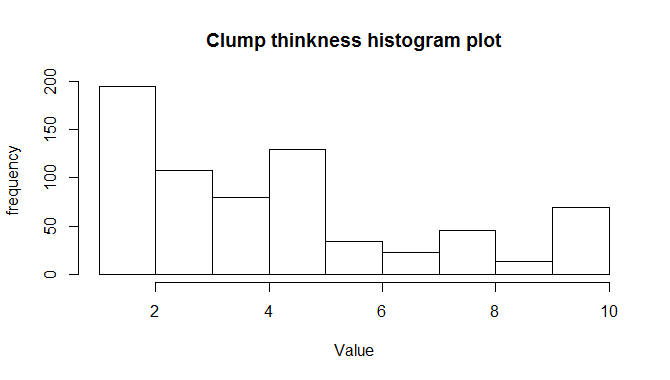
\includegraphics[width=\textwidth]{Clumpthickness.png}
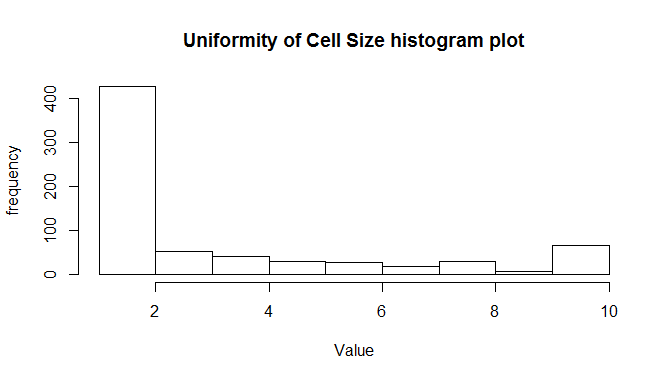
\includegraphics[width=\textwidth]{cellsize.png}
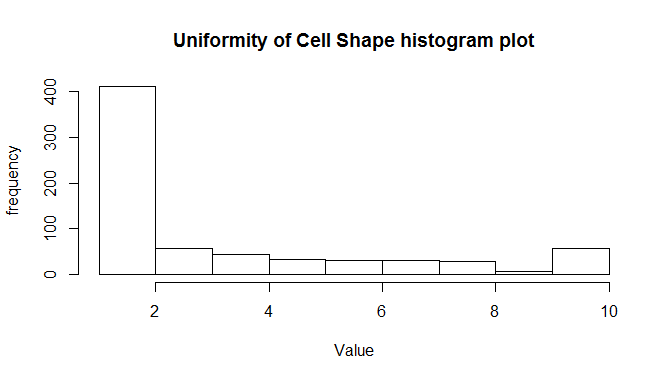
\includegraphics[width=\textwidth]{cellshape.png}
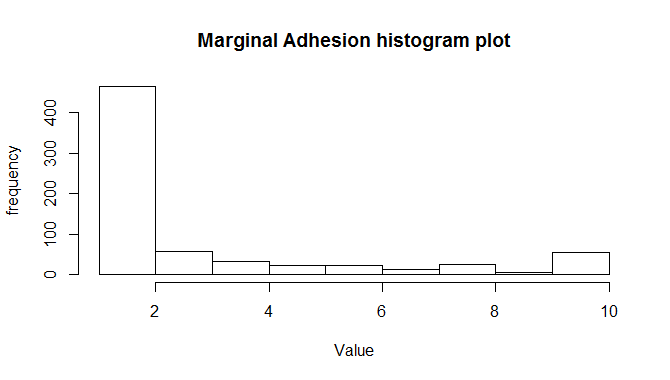
\includegraphics[width=\textwidth]{marginal.png}
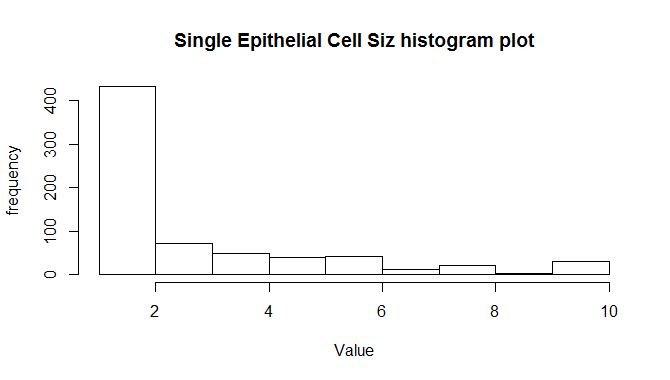
\includegraphics[width=\textwidth]{single.png}
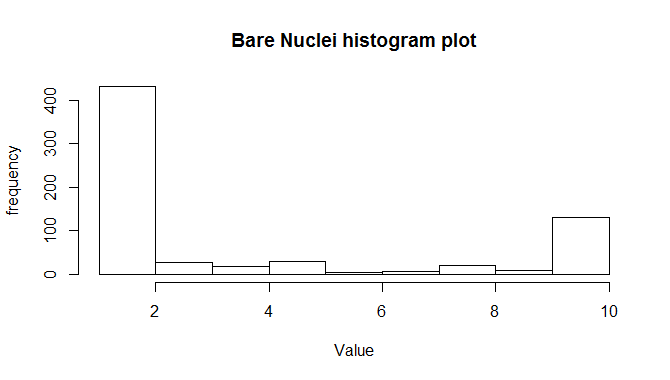
\includegraphics[width=\textwidth]{nuclei.png}
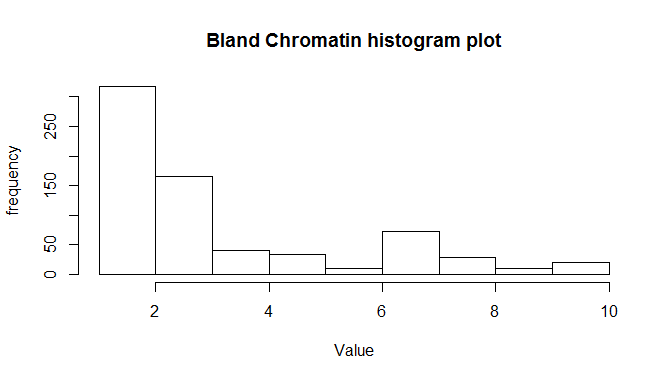
\includegraphics[width=\textwidth]{bland.png}
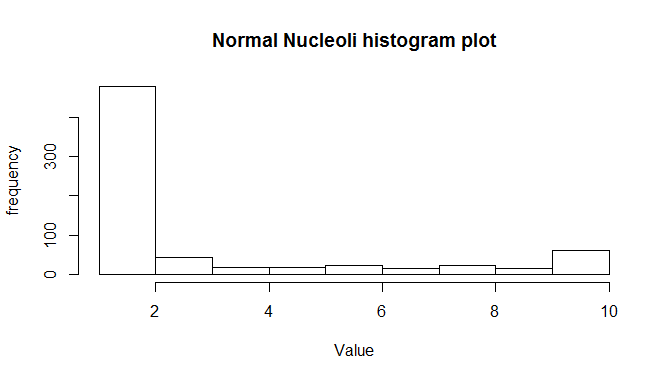
\includegraphics[width=\textwidth]{normal.png}
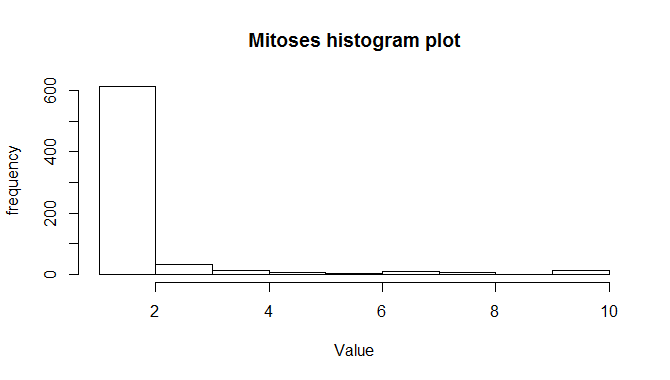
\includegraphics[width=\textwidth]{mitoses.png}
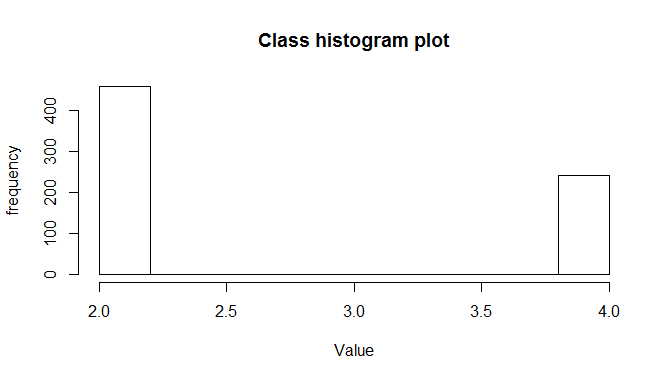
\includegraphics[width=\textwidth]{class.png}


 \item Find the mean, median, mode, and variance of each attribute. \\
 mean of each attribute can be found by using $apply(BreastCancerdata1,2,mean,na.rm=TRUE)$ in R 
 median of each attribute can be found by using $apply(BreastCancerdata1,2,median,na.rm=TRUE)$ in R
mode can be found by running
$Mode <- function(x) {
  uniquex <- unique(x)
  uniquex[which.max(tabulate(match(x, uniquex)))]
}$

$apply(BreastCancerdata1,2,Mode)$

variance can be found by using $print (var(as.matrix(BreastCancerdata1)))$

 \item For each pair $A_i, A_j$, $i \neq j$, find the Pearson's correlation coefficient. This provides an insight to the linearity of the attributes.  To remind you,
 \begin{eqnarray*}
 \rho_{X,Y} &=& \frac{\mathrm{E}[(X - \mu_X)(Y-\mu_Y)]}{\sigma_X\sigma_Y}\\
 &&\\
 &&\sigma\ \mbox{\rm is the standard deviation}\\
 && \mu\ \mbox{\rm is the mean} \\
 &&\ \mathrm{E} \mbox{\rm is the expectation}
 \end{eqnarray*}
 How is $\rho$ related to $cos \theta = \frac{\mathbf{x}\mathbf{y}}{||\mathbf{x}|| ||\mathbf{y}||}$?  Remove one of the pairs of attributes that are strongly linearly related for every pair of attributes.  Call this $\Delta_2^{clean}$.  What is the purpose of this step? \\
Running print (cor(as.matrix(meanBreastCancerdata1))) in R gives us a corelation matrix for data in meanBreastCancerdata1 dataframe. By looking at the matrix we can find that Uniformity of Cell Size and Uniformity of Cell Shape arre corelated with pearson correaltion of 0.9068819. So we can remove any of these columns. I am removing "Uniformity of Cell Size" column. When two columns are very correlated it means that these columns tell us the same thing about predicted class and there is not new information we will get by including both of these columns.
 \end{enumerate} 
  \item  Implement $k$-means so that you can cluster $\Delta_2^{clean}$ without using $C$.  Upon stopping, you will calculate the quality of the centroids and of the partition.  For each centroid $c_i$, form two counts:
  \begin{eqnarray*}
  b_i &\gets& \sum_{\delta \in c_i.B} [\delta.C = 2],\ \ \ \mbox{\rm benign}\\
  m_i &\gets& \sum_{\delta \in c_i.B} [\delta.C = 4], \ \ \ \mbox{\rm malignant}
  \end{eqnarray*}
  where $[x = y]$ returns 1 if True, 0 otherwise.  For example, $[2 = 3] + [0 = 0] + [34 = 34] = 2$
  
  The centroid $c_i$ is classified as benign if $b_i > m_i$ and malignant otherwise.  We can now calculate a simple error rate.    Assume $c_i$ is benign.  Then the error is:
 \begin{eqnarray*}
 error(c_i) &=& \frac{m_i}{m_i + b_i}
 \end{eqnarray*}
 We can find the total error rate easily:
 \begin{eqnarray*}
 Error(\{c_1, c_2, \ldots, c_k\}) &=& \sum_{i=1}^k error(c_i)
 \end{eqnarray*}

Report the total error rates for $k = 2,\ldots 5$ for 20 runs each, presenting the results that are easily understandable.  Plots are generally a good way to convey complex ideas quickly.  Discuss your results and include your initial problem statement.    \\
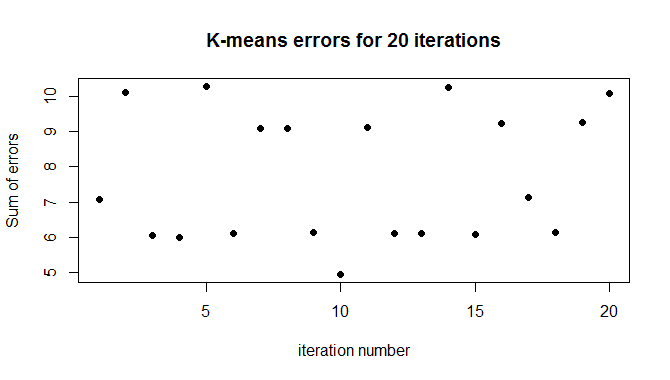
\includegraphics[width=\textwidth]{errorplot.png}
\end{enumerate}

\section*{What to Turn-in}
\begin{itemize}
\item The *pdf of the written answers to this document.
\item The code for $k$-means, \texttt{R}.
\item The AIs can schedule a time to verify your codes works.  If there is a subsequent time-stamp to the due date of the source code, the grade may be reduced.  
\end{itemize}
\bibliographystyle{unsrt} 
\bibliography{hw2}
\end{document}
